\documentclass[12pt,a4paper,ngerman]{scrartcl}

% Dateikodierung ist latin1%
\usepackage[utf8]{inputenc}
\usepackage[ngerman]{babel}
\usepackage{listings}
\usepackage[usenames,dvipsnames,svgnames,table]{xcolor}
\usepackage{verbatim} 
\usepackage{soul}
\usepackage[normalem]{ulem}
\usepackage{sectsty}
\usepackage{varwidth}
\usepackage{truncate}
\usepackage{hyperref}
\usepackage{graphicx}
\usepackage{float}
\usepackage{framed}
\usepackage{mdframed}
\usepackage{array}
\usepackage{colortbl}

\definecolor{dkgreen}{rgb}{0,0.6,0}
\definecolor{gray}{rgb}{0.5,0.5,0.5}
\definecolor{mauve}{rgb}{0.58,0,0.82}

% Setting the properties for links, urls etc.
\hypersetup{
    colorlinks,
    citecolor=black,
    filecolor=black,
    linkcolor=black,
    urlcolor=blue
}

\lstset{ %
  language=C++,                     % the language of the code
  basicstyle=\footnotesize\ttfamily,    % the size of the fonts that are used for the code
  numbers=left,                     % where to put the line-numbers
  numberstyle=\tiny\color{gray},    % the style that is used for the line-numbers
  stepnumber=1,                     % the step between two line-numbers. If it's 1, each line will be numbered
  numbersep=5pt,                    % how far the line-numbers are from the code
  backgroundcolor=\color{white},    % choose the background color. You must add \usepackage{color}
  extendedchars=true            %
  showspaces=false,                 % show spaces adding particular underscores
  showstringspaces=false,           % underline spaces within strings
  showtabs=false,                   % show tabs within strings adding particular underscores
  frame=single,                     % adds a frame around the code
  rulecolor=\color{gray},           % if not set, the frame-color may be changed on line-breaks within not-black text (e.g. comments (green here))
  tabsize=4,                        % sets default tabsize to 2 spaces
  captionpos=b,                     % sets the caption-position to bottom
  breaklines=true,                  % sets automatic line breaking
  breakatwhitespace=false,          % sets if automatic breaks should only happen at whitespace
  title=\lstname,                   % show the filename of files included with \lstinputlisting; also try caption instead of title
  keywordstyle=\color{blue},        % keyword style
  commentstyle=\color{dkgreen},     % comment style
  stringstyle=\color{mauve},        % string literal style
  escapeinside={\%*}{*)},           % if you want to add LaTeX within your code
  morekeywords={*,...}          % if you want to add more keywords to the set
}

% Color definitions
\definecolor{crucial}{RGB}{0,60,0} % This color marks the portions of code that are crucial (see below)
\definecolor{cream}{RGB}{255,255,204} % highlighting color
\definecolor{blue}{RGB}{0,0,255}

\newcommand{\hlc}[2][cream]{{\sethlcolor{#1} \hl{#2}}}

\subsectionfont{\normalsize} % We change the sections to have a slightly smaller size

% Crucial marks keywords or statements that are crucial for passing the exam ;-)
\newcommand{\crucial}[1]{\hlc[cream]{#1}} % Optimized for online reading
%\newcommand{\crucial}[1]{\textbf{\textcolor{crucial}{\uline{#1}}}} % custom
%\newcommand{\crucial}[1]{\uline{#1}} % Optimized for print

% Question Command
\newcommand{\question}[1]{
	\subsection[\truncate{0.80\textwidth}{#1}]{
	\textcolor{blue}{#1}}}

\newenvironment{multilinequestion}[1][]
	{\subsection[\truncate{0.80\textwidth}{#1}]{\textcolor{blue}{#1}} \color{blue}}
	{}

% Used for the right vertical bar next to the answer blocks
% \newlength\RightBarWidth
% \setlength\RightBarWidth{1pt}
% \newenvironment{rightbar}
% 	{
% 	\def\FrameCommand##1{%
% 	\hspace{\textwidth}\hspace{-\RightBarWidth}%
% 	{\color{dkgreen}\vrule width \RightBarWidth}
% 	\hspace{-\textwidth}##1\hfill}%
% 	\MakeFramed{\addtolength\hsize{-\width-\RightBarWidth-\columnsep}%
% 	\FrameRestore}%
% 	}
% 	{\endMakeFramed}

% Make footnotes available inside frames
\makeatletter

\newcommand\mystuff@footnotebuffer{}
\newcounter{mystuff@footnote}

\newcommand\bufferfootnotes{
	\let\mystuff@footnoteold\footnote
	\setcounter{mystuff@footnote}{\thefootnote}
	\renewcommand\mystuff@footnotebuffer{}
	\renewcommand{\footnote}[1]{
		\footnotemark
		\g@addto@macro{\mystuff@footnotebuffer}{
			\stepcounter{mystuff@footnote}
			\protect\footnotetext[\themystuff@footnote]{##1}
		}
	}
}

\newcommand\stopbufferingfootnotes{%
	\mystuff@footnotebuffer%
	\renewcommand{\footnote}[1]{\mystuff@footnoteold{##1}}%
}

\makeatother

% Answer environment
\newenvironment{answer}
                {\bufferfootnotes }
                {\stopbufferingfootnotes}
                  
\title{Technische Informatik 2 \\ Fragenkatalog \\ WiSe 2012/2013 \\[5pt] \Large{Universität Bremen}}
\date{\today}

\begin{document}

% Insert title here
\maketitle

% Abstract section
\begin{abstract}
Seit jeher gibt es auf den \textbf{Übungsblättern} des Kurses \textit{Technische Informatik 2} der Universität Bremen Zusatzfragen, die der Vorbereitung auf das \textbf{Fachgespräch} dienen sollen. Nachfolgend finden Sie die von freiwilligen Studenten und Tutoren zusammengetragenen Antworten auf diese Fragen.

\paragraph*{}
Jeder kann dazu beitragen, die Antworten zu erweitern, zu verbessern oder zu aktualisieren, indem er das Repository auf Github cloned, das Dokument überarbeitet und anschließend Merge-Requests einreicht. Das Repository befindet sich unter  \url{https://github.com/momesana/ti2-fragenkatalog/}.
\end{abstract}

\newpage

% This inserts the table of contents
\tableofcontents 

% Templates for question and answer pairs
%
% Simple question
%\question{}
%\begin{answer}
%\end{answer}
%
% Multilone question: To be used if the question contains images or blocks etc.
%\begin{multilinequestion}[text to appear in the subsection]
%\end{multilinequestion}
%the question that spans many lines
%\begin{answer}
%the answer
%\end{answer}

% This included Fragment contains questions regarding Operating Systems
\section{Betriebssysteme - Grundlagen}

\question{Welche zwei Hauptaufgaben hat ein Betriebssytem?}
\begin{answer}
    \begin{itemize}
    \item \crucial{Abstraktion von Ger"ateeigenschaften}
        \begin{itemize}
            \item Geräteunabh"angige Schnittstelle zu den Anwendungen 
            \item Geräteüberwachung und -steuerung
        \end{itemize}
    
    \item \crucial{Unterst"utzung des Mehrbenutzerbetriebs}
        \begin{itemize}
            \item Betriebsmittelverwaltung
            \item Zuteilungsstrategien
            \item Kostenabrechnung
            \item Schutz
        \end{itemize}
    \end{itemize}
\end{answer}

\question{Was ist ein Prozess?}
\begin{answer}
Ein \crucial{Programm in Ausf"uhrung}.
\end{answer}

\question{Was sind Dateien?}
\begin{answer}
Dateien sind \crucial{langlebige, "uber eindeutige Namen (Pfade) identifizierbare Datenobjekte}. Prozesse können auf sie zugreifen und sie modifizieren (wenn die nötige Berechtigung gegeben ist). Für UNIX stellt der Inhalt lediglich eine Bytefolge dar (beliebige interne Struktur).
\end{answer}

\question{Welche Arten von Dateien gibt es?}
\begin{answer}

\begin{itemize}
\item Normale Dateien (plain files)
\item Verzeichnisse
\item Symbolische Links
\item Geräte-Dateien
	\begin{itemize}
	\item Blockorientierte Gerätedateien
	\item Zeichenorientierte Gerätedateien
	\end{itemize}
\item Sockets~(\ref{netzwerke:sockets}) und Named Pipes~(\ref{netzwerke:named-pipe})
\end{itemize}

\end{answer}

\question{Wie ist ein UNIX-Dateisystem strukturiert? Wie können Dateien darin (eindeutig) aufgefunden
werden?}
\begin{answer}
Ein UNIX-Dateisystem ist eine \crucial{hierachisch organisierte} Verzeichniss-Struktur. Ganz oben steht \crucial{ die Wurzel} (root). In Vezeichnissen können Dateien abgelegt werden. Vollständige Dateinamen (absoluter Pfad) sind (eindeutige) \crucial{Pfadnamen} von der Wurzel abwärts. Relative Pfade sind ebenfalls möglich.
\end{answer}

\question{Was ist ein \textit{symbolic link} (symbolischer Link)?}
\begin{answer}
Ein \textit{ symbolic link} ist ein \crucial{Verweis auf eine Datei oder auf ein Verzeichnis} (, die nicht notwendigerweise existieren müssen). Es ist also lediglich eine Referenz auf die Zieldatei bzw. das Zielverzeichnis (d.h. ein weiterer Pfad zu einer Datei). Ein Löschen oder Verschieben der eigentlichen Datei oder das Verweisen auf eine nicht existierende Datei führen üblicherweise dazu, dass die Referenz „ins Leere“ weist \crucial{(dangling link)}.

\question{Was ist ein \textit{hard link}?}
\paragraph*{}
Ein \crucial{Hardlink} ist im Grunde genommen ein \crucial{weiterer, regul"arer Name der Datei} (Zwei Namen für die selbe Datei). Wird also die Datei unter ihrem ursprünglichen Namen gelöscht, ist sie unter ihrem zweiten Namen immer noch vorhanden. Erst wenn alle "Namen" gelöscht sind ist die Datei nicht mehr zugreifbar. Intern wird dies durch Reference-Counting erreicht. Hardlinks \crucial{k"onnen nicht auf Verzeichnisse gelegt werden} (Vermeidung unkontrollierte Schleifen).
\end{answer}

\question{Ist das UNIX-Dateisystem wirklich ein Baum? Begründung.}
\begin{answer}
Ein UNIX-Dateisystem entspricht eher einem \crucial{gerichteten Graphen} als einem Baum. Verzeichnisse und Dateien sind zwar hirarchisch organisiert, aber Möglichkeit von \crucial{Hardlinks}, d.h. das mehrfache Vorhandensein in der Dateistruktur einer physikalisch nur einfach vorhanden Datei stört das Bild eines Baumes. In einem Baum werden die Knoten benannt, unter UNIX werden Pfadnamen benutzt.
\end{answer}

\question{Welche Zugriffsrechte kann man auf eine UNIX-Datei haben? Welche Dateiattribute steuern dies, und wie?}
\begin{answer}
Die Zugriffsrechte sind \crucial{Lesen}, \crucial{Schreiben} und \crucial{Ausf"uhren}.
Es können unterschiedliche Rechte für den \crucial{Besitzer} (user) einer Datei, die \crucial{Gruppe} (group) und den \crucial{Rest der Welt} (others) festgelegt werden. Zusätzlich gibt es noch die erweiterten Rechte \crucial{Setuid}, \crucial{Setgid} und das \crucial{Sticky Bit.}\footnote{http://de.wikipedia.org/wiki/Unix-Dateirechte\#Sonderrechte.2Ferweiterte\_Rechte}

\subsection*{Detaillierte Auflistung der Zugriffsrechte:}
{\tiny\bfseries
\renewcommand{\arraystretch}{1.5}
	\begin{center}
	  \begin{tabular}{ | p{1.3cm} ||
	  >{\color{blue}\centering\arraybackslash}m{1.5cm} |
	  >{\color{blue}\centering\arraybackslash}m{1.5cm} |
	  >{\color{blue}\centering\arraybackslash}m{1.5cm} ||
	  >{\color{dkgreen}\centering\arraybackslash}m{1.2cm} |
	  >{\color{dkgreen}\centering\arraybackslash}m{1.2cm} |
	  >{\color{dkgreen}\centering\arraybackslash}m{1.2cm} ||
	  >{\color{dkgreen}\centering\arraybackslash}m{0.8cm} |
	  >{\color{dkgreen}\centering\arraybackslash}m{0.8cm} |}
	    \hline
	     
	     &  \multicolumn{3}{c||}{Erweiterte Rechte} & \multicolumn{3}{c||}{User (Owner)} & \textcolor{black}{Group} & \textcolor{black}{Others} \\ \hline
	     
	     & SUID & SGID & Sticky & r & w & x & r w x & r w x  \\ \hline
	    
	    \textbf{Plain file} & \uline{Ausf"uhren:} Benutzer vs. \uline{Besitzer der Datei} & \uline{Ausf"uhren:} Benutzer vs. \uline{Dateigruppe} & (Bleibt im Swap Space kleben) & Lesen & Schreiben & Ausführen & (dito) & (dito)  \\ \hline
	    
	    \textbf{Directory} &  & Dateien darin erhalten Gruppe der Dir & Nur eigene Dateien in Dir löschbar (bsp.: /tmp) & Einträge lesen & Einträge (indirekt) ändern & Auf Dateien darin zugreifen & (dito) & (dito)  \\ \hline
	  \end{tabular}
	\end{center}
}
\end{answer}

\question{Welche Vorteile bietet es, auf Terminals in UNIX wie auf Dateien zuzugreifen? Was versteht man unter Ein-/Ausgabeumlenkung?}
\begin{answer}
Da unter \textbf{UNIX} der Zugriff auf Geräte im allgemeinen (d.h. auch auf Terminals) als Zugriff auf eine Dateien abgebildet sind, bietet dies den Vorteil der \crucial{einheitlichen Schnittstelle und Handhabung}. Der Benutzer
kann auf das Terminal zugreifen wie auf eine Datei auch und muss sich daher nicht mit den konkreten Geräteeigenschaften auseinandersetzen. \\
Es gibt \crucial{Standardein- und Standardausgaben von Prozessen}. Will der Benutzer andere Ein- bzw. Ausgabemöglichkeiten nutzen, kann er Ein- und Ausgaben umlenken. Beispielsweise können die Fehlermeldungen in eine Datei umgelenkt werden.

%% Bash script
\lstset{language=bash,caption={Ein-/Ausgabeumlenkung}}
\begin{lstlisting}
user $ echo -e "#\!/bin/bash\necho Hello world" > /tmp/bla # (1)
user $ bash < /tmp/bla # (2)
Helloworld
\end{lstlisting}

\begin{enumerate}
\item Die Ausgabe des Befehls \texttt{echo} wird in eine Datei \texttt{/tmp/bla} geschrieben, und somit eine Ausgabeumlenkung getätigt.

\item Unter (2) liest die neu erzeugte shell von der soeben erstellten Datei \texttt{/tmp/bla} anstelle des Terminal, was einer Eingabeumlenkung entspricht.
\end{enumerate}

\end{answer}

\question{Welche Aufgabe hat ein Kommando-Interpreter (z.B. in UNIX die Shell)?}
\begin{answer}
Ein Kommando-Interpreter stellt dem Benutzer eine einfache (und zugleich mächtige) Schnittstelle zum Betriebssystem \crucial({Benutzungsschnittstelle}) zur Verfügung. Damit lassen sich Aufträge an das Betriebssystem absetzen. Die Shell ist ebenfalls ein Prozess.
\end{answer}

\question{Was machst Du, wenn Dir die genaue Semantik eines Unix-Kommandos entfallen ist?}
\begin{answer}
Zunächst die Hilfe (mit dem \crucial{Kommandozeilenswitch --help}), und wenn erforderliche die \crucial{Man-} oder \crucial{Infopages} zur Rate ziehen:
%% Bash script
\lstset{language=bash,caption={Hilfe zu einem Kommando am Beispiel von \texttt{mkdir}}}
\begin{lstlisting}
user $ mkdir --help
user $ man mkdir
user $ info mkdir
\end{lstlisting}
\end{answer}

\begin{multilinequestion}[\texttt{bla} sei ein ausführbares Programm. Was ist der Unterschied zwischen dem Aufruf]

%% Bash script
\lstset{caption={}}
\begin{lstlisting}
bla
\end{lstlisting}

und dem Aufruf

%% Bash script
\lstset{caption={}}
\begin{lstlisting}
bla &
\end{lstlisting}

in der Shell? Welche Auswirkungen hat dies, wenn \texttt{bla} von \textbf{Standard Input} liest bzw. auf \textbf{Standard Output} schreibt?
\end{multilinequestion}

\begin{answer}
\texttt{bla} wird im \crucial{Vordergrund} ausgeführt und beansprucht das Terminal (=Tastatur) für sich. Weitere Shell-Eingaben sind daher erst möglich, nachdem \texttt{bla} terminiert.

\paragraph{}
Hängt man einem Befehl ein \& an, so wird dieser im \crucial{Hintergrund} ausgeführt (Hintergrundprozess). Er gibt damit die Kontrolle über das Terminal auf, so dass dieses für neue Prozesse verwendet werden kann. Dieser \crucial{kann} dann zwar auf \texttt{stdout} \crucial{schreiben}, wird aber sofort in den Zustand \crucial{suspended} versetzt , \crucial{wenn er versucht von der Standardeingabe (\textit{stdin}) zu lesen}.
\end{answer}

\begin{multilinequestion}[Prozessbäume: Gegeben sei der folgende Prozessbaum:]

\begin{figure}[H]
  \caption{Prozessbaum}
  \centering
    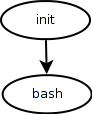
\includegraphics[scale=0.70]{images/process-tree01}
\end{figure}

Wie ändert er sich nach Eingeben der folgenden Kommandofolge im Shell?

%% Bash script
\lstset{language=bash,caption={Eingegebene Befehle}}
\begin{lstlisting}
sleep 1000 &
emacs &
bash
date
\end{lstlisting}

\end{multilinequestion}

\begin{answer}
Der Prozessbaum sieht nach Eingabe der obigen Befehle folgendermaßen aus:
\begin{figure}[H]
  \caption{Prozessbaum nach den Eingaben}
  \centering
    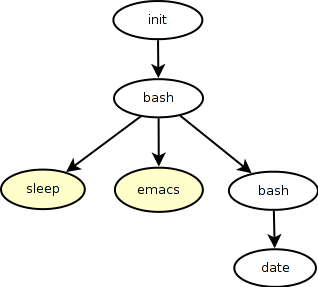
\includegraphics[scale=0.70]{images/process-tree02}
\end{figure}
\texttt{sleep} und \texttt{emacs} laufen dabei als Hintergrundprozesse.
\end{answer}


\question{Nenne drei Beispiele für Informationen, die der Betriebsystemkern über einen Prozess wissen muss.}
\begin{answer}
\begin{itemize}
\item \crucial{Prozess ID}
\item \crucial{Parent-Prozess ID}
\item \crucial{Zustand des Prozesses}
\end{itemize}

\end{answer}

\question{Was ist eine Pipe?}
\begin{answer}
Eine Pipe ist die \crucial{Umlenkung} eines \crucial{unidirektionalen sequentiellen Bitstroms} von der \crucial{Standardausgabe} eines Prozesses auf die \crucial{Standardeingabe} eines Prozesses.
\end{answer}

\question{Wie macht man ein soeben editiertes Shell-File ausführbar?}
\begin{answer}
\crucial{Setzen des Ausf"uhrbar-Bits} (executable bit) (x). \\

%% Bash script
\lstset{language=bash,caption={Setzen des \textbf{executable bit} für ein Shellskript \textit{shellfile.sh}}}
\begin{lstlisting}
chmod +x shellfile.sh
\end{lstlisting}

\end{answer}

\question{In welche Bereiche (Segmente) ist der virtuelle Adressraum eines Programmes in Ausführung unter UNIX unterteilt, und welche Eigenschaften kennzeichnen sie?}
\begin{answer}
Der virtuelle Adressraum ist in \crucial{Text}, \crucial{Data} und \crucial{Stack} unterteilt. Im Text-Teil befindet siche
der eigentliche Programmcode, im Data-Teil die Daten und auf dem Stack alle temparären
Daten (z.B. Variablen).
\end{answer}

\question{Wozu wird der Stack verwendet?}
\begin{answer}
Auf einem Stack werden die \crucial{innerhalb von Funktionsaufrufen tempor"ar anfallenden Daten eines Prozesses} abgelegt. Das umfasst unter anderem die Rücksprung-Addresse, die an die Funktion übergebenen Argumente und lokale Variablen.
\end{answer}

\question{Welchem Zweck dienen Bibliotheken (Libraries)?}
\begin{answer}
Bibliotheken \crucial{stellen Funktionen zur Verf"ugung}. Durch das Vorhandensein von Bibliotheken muss ein Programmierer nicht von Grund auf alle Funktionen neu schreiben.

\paragraph{}
Eine Programmbibliothek bezeichnet in der Programmierung eine \crucial{Sammlung von Softwaremodulen}, die Lösungswege für thematisch zusammengehörende Problemstellungen anbieten. Bibliotheken sind im Unterschied zu Programmen keine eigenständig lauffähigen Einheiten, sondern Hilfsmodule, die von Programmen angefordert werden.\footnote{http://de.wikipedia.org/wiki/Programmbibliothek}

\end{answer}

\question{Welche Aufgabe erfüllt ein Linker?}
\begin{answer}
Ein Linker oder Binder verbindet einzelne Programmmodule zu einem ausführbaren Programm. Im Zuge dessen werden die Symbole in den Objectfiles aufgelöst. Man unterscheidet zwischen statisches und dynamisches Linken. Man unterscheidet dabei zwischen \crucial{statisches und dynamisches Linken}.

\paragraph*{Statisches Linken:}
Die Symbole schon während des Zusammenstellens der Programmdatei aufgelöst

\paragraph*{Dynamisches Linken:}
Das Auflösen der Symbole erfolgt erst bei der tatsächlichen Ausführung des Programms.
\end{answer}

\question{Wozu wird beim Assemblieren eine Symboltabelle angelegt?}
\begin{answer}
Zum Auflösen von Verweisen.
\end{answer}

\question{Welchen Vorteil hat es, Bibliotheken mit \textit{Position Independent Code} zu versehen?}
\begin{answer}
Position-independent Code (PIC, engl. für positionsunabhängiger Code) ist \crucial{Maschinencode, der ausgef"uhrt werden kann, unabh"angig davon, an welcher absoluten Adresse im Hauptspeicher er sich befindet}. PIC wird üblicherweise für dynamische Bibliotheken verwendet, damit diese für jedes Programm an eine Speicherposition geladen werden können, wo sie sich nicht mit anderen Objekten dieses Programms überlappen.\footnote{http://de.wikipedia.org/wiki/Position-Independent\_Code} 
\end{answer}

\question{Durch welche "Qualitätsmerkmale" sollten Betriebssysteme gekennzeichnet sein? Nenne Beispiele für konkurrierende Anforderungen.}
\begin{answer}
\crucial{Effizienz, Kosten, Bedienbarkeit, Zuverl"assigkeit, Verf"ugbarkeit, Sicherheit, Wartbarkeit.
Der Kostenpunkt kann mit jeder anderen Anforderung konkurrieren.} Je besser ein Aspekt werden soll, desto mehr Zeit und Entwicklungsarbeit, sprich Geld muss in diesen Aspekt investiert werden. Am Beispiel Windows lässt sich wunderbar erkennen, wie \crucial{Bedienbarkeit und Zuverl"assigkeit im Widerspruch} zueinander stehen können. Die Sicherheit eines OS's lässt sich oft auch nicht mit einer ausgereiften Bedienbarkeit vereinbaren, oder umgekehrt, siehe Win vs. Linux.
\end{answer}

\question{Worin unterscheidet sich der Kernel-Mode vom User-Mode (in UNIX)? Warum wird diese Unterscheidung getroffen?}
\begin{answer}
\crucial{Kernel und Useradressraum sind aus Sicherheitsgr"unden getrennt. Im User-Mode gibt es keinen direkten Zugriff auf die Hardware.} Das hat auch seinen Sinn, da diese Zugriffe kontrolliert erfolgen sollen, damit das System sicher und zuverlässig bleibt.
\end{answer}

\question{Was passiert etwa bei einem System-Aufruf? (Reihenfolge der Arbeitsschritte.)}
\begin{answer}
\crucial{Es erfolgt ein Trap, darauf wird der Zustand des Systems gesichert, dann erfolgt der Sprung in den Kernel-Mode, in dem der eigentliche Hardware-Zugriff erfolgt. Daraufhin gibt es eine R"uckmeldung und einen R"ucksprung zum Prozess, wo dann auch der Kontext wieder hergestellt wird.}
\end{answer}

\question{Was ist ein Interrupt? Nenne Beispiele für mögliche Interrupt-Quellen. Warum werden sie unterschiedlich priorisiert? Wie wird ein Interrupt in etwa behandelt?}
\begin{answer}
Ein Interrupt ist eine externe Unterbrechung eines Prozesses. Eine Quelle kann z. Bsp. die
Hardware sein. Hardwareinterrupts haben generell eine höhere Priorität als Softwareinterrupts.
Beim Clock-Tic ist die Quelle eben die Hardware, und der Prozess hat eine sehr hohe
Priorität, da ansonsten die System-Uhr nicht mehr genau laufen würde, was sich fatal auf
andere Programme auswirken kann, die sich nach dieser Uhr zu richten haben.
Beispiele für einen Softwareinterrupt wären SIGKILL oder SIGSTOP.
\end{answer}

\question{Was ist ein Trap? Nenne Beispiele. Inwiefern unterscheiden sich Traps von Interrupts?}
\begin{answer}
Ein Trap ist ein interne Unterbrechung eines Programms in Ausführung, die vom System
kommt. Beim Trap wird in den Kernel-Mode gewechselt, da es ja ein Systemaufruf ist.
Die Regelung erfolgt durch den Trap-Handler, der bei Bedarf dann auch Signale senden
kann. Division durch 0 wäre ein solches Beispiel. Es wird ein Trap ausgelöst, der durch den
Trap-Handler gejagt wird, welcher wiederum das Signal sigfpe lossendet (SignalFloating-
PointError). Die Folge ist, wie bei vielen anderen Signalen auch, dass der Prozess terminert
oder gekillt wird.
\end{answer}

\question{Was ist ein Signal? Nenne Beispiele für mögliche Signalquellen. Wie kann ein Prozess auf ein Signal reagieren?}
\begin{answer}
Signale dienen der Meldung (von Ausnahmezust"anden) an einen Prozess. Sowohl der Benutzer als auch Prozesse können Signale an Prozesse senden. Beispiele für Signale sind u.a. Stop (SIGINT), Kill (SIGKILL), Terminate und (SIGTERM). Der Traphandler ist oft eine Signalquelle.
\end{answer}

\question{Beschreibe kurz einige Zustände, in denen sich ein (UNIX-)Prozess befinden kann.}
\begin{answer}
\subsection*{Einfaches Modell:}
\begin{itemize}
\item Ready
\item Run
\item Sleep
\item Zombie
\end{itemize}


\subsection*{Erweitertes Modell:}

\begin{description}
\item[dead]\hfill \\ Der Prozess wurde beendet, er belegt jedoch noch Speicherplatz.

\item[ready]\hfill \\ Der Prozess wartet auf Zuteilung der CPU (Zeitschlitz). Gibt es den Ready-Zustand, so befinden sich höchstens so viele Prozesse im Zustand running, wie CPUs vorhanden sind.

\item[running]\hfill \\ Entweder genau der Prozess, der gerade bearbeitet wird, oder alle Prozesse, die momentan Rechenarbeit verrichten können.

\item[sleep]\hfill \\ Der Prozess wurde auf eigenen Wunsch zurückgestellt. Er kann Signale entgegennehmen, wie z. B. Timer, oder Ergebnisse von Kindprozessen.

\item[trace]\hfill \\ Der Prozess wurde von außen angehalten, üblicherweise durch einen Debugger.

\item[wait]\hfill \\ Der Prozess wartet auf ein Ereignis, üblicherweise eine Benutzereingabe.

\item[uninterruptible sleep]\hfill \\ Der Prozess wartet auf ein Ereignis, üblicherweise Hardware. Tritt dieses Ereignis ein, ohne dass der anfragende Prozess es entgegennimmt, so kann das System instabil werden.

\item[zombie]\hfill \\ Der Prozess wurde beendet und aus dem Arbeitsspeicher gelöscht, aber noch nicht aus der Prozessliste entfernt.
\end{description}

\end{answer}

\question{Nenne einige Randbedingungen, auf die man beim Entwurf eines Schedulers achten sollte. Wie sollten rechenintensive bzw. Ein-/Ausgabe-intensive Prozesse dabei behandelt werden?}
\begin{answer}
Ein Scheduler soll schlank (effizient) und fair sein, d. h. der Rechenaufwand der Prozessverwaltung
darf nicht so gross werden, dass die Effizienz darunter leidet, und jeder Prozess soll
gerechterweise auch drankommen. Auch die Zeitscheiben sollen eine angemessene Grösse
haben.
\end{answer}

\question{Wie könnte man mit Hilfe eines Round-Robin-Schedulers Prozess-Prioritäten "simulieren"?}
\begin{answer}
Man könnte die Anzahl der Durchläufe für die Prozesse mit einer hohen Priorität erhöhen,
so dass diese in einem Durchlauf mehrere Male dran kommen, oder man gibt den wichtigen
Prozessen grössere Zeitscheiben, um ihnen mehr CPU-Zeit zukommen zu lassen.
\end{answer}

\question{Warum bestehen die \textit{Sleep}- und die \textit{Run-Queue} in UNIX nicht aus jeweils einer einzigen Warteschlange? Wie sind sie stattdessen organisiert?}
\begin{answer}
Sleep-Queue und Run-Queue bestehen aus jeweils einem Array. Jede Priorität hat darin
eine eigene Liste, das Handling zwischen den Queues ist abhängig von der Priorität. Diese
Aufteilung besteht, da sonst immer alles durchsucht werden müsste.
\end{answer}

\question{Warum werden die Zustandsinformationen eines UNIX-Prozesses teilweise in der \textit{Proc-Struktur} und teilweise in der \textit{User-Struktur} abgelegt? Nenne jeweils drei charakteristische Beispiele für Angaben darin.}
\begin{answer}
Die in der Proc-Struktur abgelegten Zustandsinformationen sind für alle Prozesse verfügbar,
die in der User-Struktur abgelegten sind nur für den laufenden Prozess verfügbar.
Beispiele für Angaben in der Proc-Struktur:
Signale, die zur Verarbeitung anstehen
Prozesszustände
Scheduling
Beispiele für Angaben in der User-Struktur:
Zugriffsrechte
Aktuelles Verzeichnis
Geöffnete Dateien.
\end{answer}

\question{Skizziere kurz die Prozesserzeugung in UNIX. Welche Rolle spielen die Systemaufrufe fork() und exec() dabei?}
\begin{answer}
Der Prozess Nummer Eins (INIT) wird "von Hand" beim Systemstart erzeugt.
Andere Prozesse werden bei Bedarf als Kindprozesse mit fork() (oft als Kind-Prozesse
der Shell) erzeugt. So entsteht eine Hierachie von Prozessen. Der Kindprozess erhält eine
neue Prozess-ID, ist aber zunächst eine Kopie des Vaters, d.h. der"gleiche" Adressraum
mit gleicher Aufteilung von Text, Data und Stack. Normalerweise soll das Kind ein anderes
Programm ausführen, dieses wird mit exec() gestartet, damit wird dann auch der
Adressraum ausgetauscht.
\end{answer}

\question{Wie erfährt ein UNIX-Prozess, ob ein Kindprozess terminiert ist? Wozu gibt es in UNIX den Prozesszustand SZOMB ("Zombie")?}
\begin{answer}
Das Kind meldet bei der Termination das Signal SIGCHILD an den Vater, dieser behnadelt
durch den Aufruf wait() den Kindprozess und der Kindprozess terminiert
oder der Vater ignoriert das Signal. In diesem Fall wird das Kind zum Zombie. Der Zombie
wird dann entweder später vom Vater behandelt oder (je nach UNIX-Variante) durch das
Betriebssystem. Z.B. kann der INIT-Prozess die Proc-Struktur wieder freigeben.
\end{answer}

\question{Welche Vor- und Nachteile hat der First-Fit- bzw. der Best-Fit-Algorithmus zur Speicherverwaltung? Wie funktioniert der Buddy-Algorithmus in etwa?}
\begin{answer}
First-Fit-Algorithmus:
Der erste Block, der gross genug ist, wird verwendet indem er in zwei Teile gespalten wird
(gross genug für die Anforderung und Rest).
Das führt zu einer Ansammlung von kleinen Blöcken am Anfang der Liste, es werden immer
mehr Blöcke und sie werden im Mittel immer kleiner. Das führt zu im Mittel längerer
Suche, kleine Anforderungen können schnell erfüllt werden.
Best-Fit-Algorithmus:
Die Liste wird immer ganz durchsucht, der Block mit dem kleinsten Verschnitt wird ausgew
ählt.
Es entstehen extrem viele kleine Blöcke. Die Suche dauert sehr lange da immer die ganze
Liste durchsucht wird. Es sind lange auch grosse Blöcke verfügbar.
Buddy-Algorithmus:
Blöcke sind immer 2k gross. Bei der Freigabe eines Blockes wird er, wann immer sein
Nachbar (Buddy) frei ist, mit dem Nachbarn verschmolzen.
Das vereinfacht das splitten und zusammenfügen der Blöcke. Allerding entsteht freier Speicher
innerhalb der Blöcke.
Optimierung: mehrere Listen mit jeweils gleich grossen Blöcken, das verringert die Suchdauer.
\end{answer}

\question{Wozu bieten Systeme eine Speicherhierachie an? Welche Beobachtung über den Speicherzugriff realer Programme liegt dem zugrunde? Welche verschiedenen Arten von Speicher werden typischerweise bereitgestellt?}
\begin{answer}
Die Systeme bieten eine Speicherhierachie an da die Geschwindigkeit sich konträr zu den
Kosten verhält. Reale Programme greifen oft nur auf eine sehr kleine Bereich zu (Working Set). Es werden meist Cache, Hauptspeicher und Massenspeicher bereitgestellt.
\end{answer}

\question{Warum ist es in der Regel nicht sinnvoll, den Adressraum eines Prozesses in einem Stück im Speicher abzulegen?}
\begin{answer}
Ein Prozess muss nicht zwangsläufig komplett im Speicher verfügbar sein (s.o.:Working
Set). Bei der Aufteilung in kleinere Einheiten ist auch die Nutzung kleinerer Freispeichereinheiten möglich, heisst insgesamt eine erheblich bessere Nutzung des Haupspeichers.
\end{answer}

\question{Was versteht man unter \textit{Paging}, was unter \textit{Segmentierung}? Wo tritt \textit{interne Fragmentierung}, wo \textit{externe Fragmentierung} auf? Was versteht man darunter?}
\begin{answer}
Segmentierung:
Speicher wird in verschieden grosse Stücke unterteilt, das ermöglicht die 
exible Zuteilung
kleiner Speicherbereiche und Shared Memory.
Es sind Adressumsetzungstabellen pro Prozess notwendig.
Segmente enthalten unterschiedlich viele Pages und sind maximal 210Bytegross:
Paging:

exible Zuteilung von gleich grossen Speichereinheiten. Der Hauptspeicher wird in Kacheln (PageFrames)
fester Grösse unterteilt, die Prozessadressräume wiederum liegen in Seiten (Pages) von
gleicher Grösse. Auch dieses Verfahren ermöglicht Shared Memory, impliziert aber interne Fragmentierung.
externe Fragmentierung: wenn durch die angewendete Logik Speicher in unterschiedlich grosse
Stücke eingeteilt wird und ganze Stücke freibleiben.
interne Fragmentierung: wenn innerhalb von gleich grossen Stücken der Speicher nicht restlos
ausgenutzt wird und so Speicher ungenutzt bleibt.
\end{answer}

\question{Aus welchen Teilen besteht eine \textit{virtuelle Adresse} zumeist? Wie ermittelt sich daraus die entsprechende Hauptspeicheradresse, d.h. wie läuft die Adressverwaltung in etwa ab?}
\begin{answer}
Eine virtuelle Adresse besteht zumeist aus zwei Teilen: jPAGEjADDRj. Der erste Teil wird bei Gebrauch in der Page-Tabelle "nachgeschaut" und entsprechend ersetzt: jADDRjADDRj.
Dieser Vorgang wird üblichwerweise durch Hardwareunterstützung realisiert: die Memory-Managment-Unit (MMU).
\end{answer}

\question{Wie können mehrere Prozesse mit Hilfe virtueller Adressierung auf dieselben Programmstücke (oder auch Datenbereiche) zugreifen?}
\begin{answer}
Shared Memory:
In den jeweiligen (unterschiedlichen) Page-Tabellen sind dieselben Seiten eingetragen. (Doppelter bzw. dreifacher Eintrag ein und desselben Inhalts in die 'Inhaltsverzeichnisse').
\end{answer}

\question{Wie arbeiten die folgenden Algorithmen zur Verdrängung von Seiten aus dem Hauptspeicher in etwa?}
\begin{answer}
LRU (Least-Recently-Used)
LRU entfernt die Seite im Hauptspeicher, auf die am längsten nicht mehr zugriffen
wurde. Das Lokalitätsprinzip wird in der Regel gut erfasst. LRU besitzt eine gute
Aproximation an den optimalen Algorithmus,
aber das erfassen aller Zugriffszeiten auf die Seiten ist notwendig, d.h. bei jedem
Zugriff müssen weitere Speicherzugriffe erfolgen. LRU ist zu aufwendig ohne Spezialhardware.

FIFO (First-in-First-Out)
FIFO entfernt die älteste Seite und ist einfach zu realisieren: als verkettete Liste der
Page Frames nach Belegungsalter.
Aber: bestimmt das Working Set in der Regel nicht gut.

Second-Chance-FIFO
Funktioniert (im Prinzip) wie FIFO: als verkettete Liste nach Belegungsalter. Wenn
eine Seite (nach FIFO) zum Löschen an der Reihe ist wird überprüft ob sie seit
ihrer letzten überprüfung referenziert wurde. Wenn ja: sie wird wieder (als jüngste
Seite) in die Liste eingehängt. Wenn nein: löschen der Seite.
In diesem Algorithmus wird unterschiedliche Benutzungshäufigkeit einkalkulliert,
aber er ist sehr aufwendig, da auch eine FIFO-Liste geführt werden muss (s.o.)

NRU (Not-Recently-Used)
NRU trifft eine zufällige Auswahl aus den kürzlich nicht referenzierten Seiten (z.B.
mit zyklischer Suche nach Page Frame-Nummern). Der gewählte Modus des zurücksetzens
des Referenzbits entscheidet über die Güte".
Mögliche Optimierung:
Unterscheidung zwischen Nur-Lese-Zugriffen und Schreib-Zugriffen, wird in Dirty-
Bit (D) = Modifikationsbit (M) angegeben.
Da bei kürzlich beschriebenen Seiten der veränderte Seiteninhalt erst gerettet werden
muss, sollte wegen des Aufwandes eher eine Seite mit Nur-Lese-Zugriffen zum
überschreiben gwählt werden.

Bei Lastspitzen summiert sich die Verdrängung von beschriebenen Seiten, daher
wird NRU oft nicht verwendet.
Aging
Beim Aging altern die Seiten duch shiften eines Schieberegisters das für jede Seite
angelegt wird. Das führt zu einer guten Annäherung an LRU, aber auch zu unbertretbar
hohem Aufwand. Bei Vereinfachung des Algorithmus (z.B. von Schieberegister
mit 8 Bit auf 2 Bit) gehen die LRU-ähnlichen Vorteile verloren und Aging wird
zu komplexen Variante von Second-Chance-FIFO.
\end{answer}

\question{In welche dieser Kategorien kann man den Clock-Hand-Algorithmus einordnen?}
\begin{answer}
LRU (ohne Dirty-Bit)
\end{answer}

\begin{multilinequestion}[Warum ist ein perfekter Algorithmus zur Verdrängung von Pages aus dem Hauptspeicher nicht realisierbar?]
Wie arbeiten die folgenden Algorithmen in etwa:
\begin{enumerate}
\item FIFO (First-In-First-Out),
\item LFU (Least-Frequently-Used),
\item LRU (Least-Recently-Used)?
\end{enumerate}
In welche dieser Kategorien kann man NRU (Not-Recently-Used) einordnen? Wie arbeitet
der Clock-Hand-Algorithmus?
\end{multilinequestion}

\begin{answer}
Ein optimaler Algorithmus ist für ein 'normales' Betriebssystem nicht realisierbar, da die Prozesse
durch unterschiedliche Working Sets eine unterschiedlich grosse Anzahl von Seiten unterschiedlich
lange benötigen.
Im Gegensatz dazu ist bei einem Betriebssystem mit wenigen, speziellen Aufgaben (Embeded
Systems) ein optimaler bzw. annähernd optimaler Algorithmus möglich.
\end{answer}

\question{Was passiert, wenn die Umlaufzeit des Zeigers beim Clock-Hand-Algorithmus zu gross bzw. zu klein gewählt wird? Wie kann ein zweiter Zeiger den Algorithmus verbessern?}
\begin{answer}
Wenn die Umlaufzeit zu gross gwählt wird ist irgendwann kein freier Speicher mehr verfügbar (die Freispeichereserve leer). Wird die Umlaufzeit zu klein gewählt, werden die Seiten vor ihrer nächsten Benutzung aus dem Speicher entfernt und müssen dann erneut geladen werden, die Freispeicherreserve ist grösser als sinnvoll.

\paragraph*{}
Ein zweiter Zeiger verbessert den Clock-Hand-Algorithmus insbesondere bei grossen Mengen von Speicher. Z.B. kann der erste Zeiger das Referenzbit gegebenenfalls zurücksetzen, der Zweite die
Seiten entfernen falls sie in der Zwischenzeit nicht erneut referenziert wurden.
\end{answer}

\question{Was ist Swapping? Warum wenden auch Paging-Systeme häufig dieses Verfahren an bzw. Unter welcher Bedingung?}
\begin{answer}
Swapping wird angewandt, wenn die Working Sets der aktiven Prozesse nicht vollständig in den Speicher passen. Dadurch entsteht eine hohe Page Frame-Rate, das so genannte Seiten-Flattern. Da das Lesen von der Festplatte recht lange dauert, sinkt die Geschwindigkeit, in der die Instruktionen abgearbeitet werden können, rapide.

\paragraph*{}
Durch Swapping werden nicht nur Teile von Prozessen (Paging), sondern ganze Prozesse auf die Platte ausgelagert. Längere Zeit inaktive Prozesse werden aus dem Hauptspeicher entfernt, um dort Platz verfügbar zu machen, dadurch wird natürlich ein Austausch der Prozesse im Hauptspeicher nach gewisser Zeit erforderlich.
\end{answer}

\question{Wie kann man die Vorteile von Paging und Segmentierung kombinieren?}
\begin{answer}
Bei einem einzigen Adressraum kann dieser beim Paging nicht logisch aufgeteilt werden. Der gesamte Adressraum wird in gleich grosse Kacheln eingeteilt.
Deswegen wird heute der Speicher häufig in mehrere Segmente unterteilt, die jeweils eigene Pagetabellen enthalten. Die Grösse der Segmente ist nicht statisch, sondern kann jede Gösse mit n multipliziert mit Page Frame Grösse umfassen.

\paragraph*{}
Dadurch entstehen dreiteilige Adressen:
Region mit eigener Pagetabelle, Page in der Region, Adresse in Page.
Regionen folgen dabei der logischen Grösse des Adressraumes (Text, Data, Stack), Pages sind in feste Grössen unterteilt.
\end{answer}

\question{Wozu bzw. wo wird bei der Speicherverwaltung häufig ein \textit{Assoziativspeicher} eingesetzt?}
\begin{answer}
Assoziativspeicher wird im allgemeinen als Spezialhardware innerhalb der MMU (Memory-Managment-Unit) realisiert. D.h. Assoziativspeicher == Hardware-Cache.
Er wird häufig zur Adressumsetzung genutzt. Für die gesamte Pagetabelle wäre dies sehr teuer, deswegen wird beim Prozesswechsel neu geladen, es sind (getreu dem Lokalitätsprinzip) immer nur einige Seiten in Gebrauch. Daher enthält der Cache jeweils nur diese Seiten.

\paragraph*{}
Ablauf: Adresszugriff,
Page Table Entry im Cache? Wenn ja: Adressumsetzung, wenn nein: Nachladen aus der Pagetabelle.
Es ist der parallele Zugriff auf alle im Cache befindlichen Einträge möglich. Die gesamte Pagetabelle im Hauptspeicher vorzuhalten, wäre zu langsam, da zusätzlicher Speicherzugriff nötig wäre.
\end{answer}

\question{Beschreibe kurz die Zugriffsoperationen open(), close(), lseek(), read() und write() auf ein UNIXFilesystem. Welche Rolle spielt der Filedeskriptor dabei?}
\begin{answer}
open()
Öffnet eine Datei für die weitere Arbeit. open() werden die Parameter path (Pfadname der Datei),

ags (erlaubte Folgeoperationen wie lesen, schreiben,...) und mode (Zugriffsrechte bei einer NEU
angelegten Datei) übergeben. Der File Descriptor wird zurückgegeben.
close()
Dieser Systemaufruf gibt eine Datei wieder frei.
create()
Es wird mit den Parametern path und mode eine neue Datei erzeugt. Der File Descriptor wird
zurückgegeben.
lseek()
wird mit den Parametern File Descriptor, offset und whence aufgerufen. Die aktuelle Position im
File Descriptor wird um offset Bytes gemäss whence verschoben (d.h. 0 = vom Anfang, 1 = vom
Ende, 2 = von der aktuellen Position aus).
Zusammengefasst: lseek setzt den Zeiger, der innerhalb einer Datei die Position anzeigt.
read()
mit den Parametern File Descriptor (fd), buf und len liest von len Bytes ab der aktuellen Position
des fd in den Puffer buf, dabei wird die aktuelle Position um die gelesenen Bytes weitergeschoben.
read() liefert die Anzahl der tatsächlich gelesen Bytes.
write()
mit den Parametern fd, buf und len funktioniert analog zu read() und liefert die Anzahl der geschriebenen
Bztes zurück.
\end{answer}

\question{Wie sieht die Struktur des UNIX-V7-Dateisystems auf der Platte in etwa aus? Warum erfolgt die Verwaltung der Freispeicherliste über \textit{Indirekt}-Blöcke?}
\begin{answer}
Das Dateisystem V7:
- Der Dateiinhalt ist Block-orientiert mit speziellem Block-Index organisiert.
- Der Boot-Block ist Block 0 des Root-Dateisystems und wird beim booten geladen.
- Der Superblock enthält die Verwaltungsinformationen des Dateisystems: Grösse, Verwaltung der
freien Inodes, Verwaltung der freien Blöcke (mit verketteter Liste von Blöcken mit freien Blocknummern)
- Inodes dienen zur Ablage der Verwaltungsinformationen der Dateien. Jede Datei hat einen Inode
mit:
+ eindeutigem Bezeichner (heisst: Inodenummer, diese gibt die Position an)
+ Besitzer (nid), Gruppe (gid)
+ Zeitpunkt der letzten änderung, des letzten Zugriffs, ...
+ Anzahl der Hard Links (mehrere Namen für eine Datei verweisen auf denselben Inode)
+ Anzahl von Bytes
+ Dateityp
+ Verweise auf Datenblöcke
+ Zugriffsrechte
Kleine Dateien bis zu zehn Blöcken werden direkt im Inode-Block gespeichert.
- In Indirekten Blöcken sind alle Dateien grösser als zehn Blöcke organisiert. Jeder Indirekt Block
hat auch ist auch in den Inodes mit einem Eintrag vorhanden. Mit Indirekten Blöcken sind grosse
Dateien realisierbar, mit maximal vier Zugriffen für einen Dateiblock.
Die Aufteilung in verschiedene Blöcke dient insbesondere der Sicherheit, so wird z.B. der Superblock,
ohne den der Rest des Systems nicht mehr zugreifbar ist, mehrfach an verschiedenen Stellen
der Platte gespeichert. So können die wichtigsten Informationen bei der Zerstörung des Original-
Superblockes wiederhergestellt werden. Des weiteren können durch Verschleiss kappute Blöcke als
nicht benutzbar deklariert werden. Das Gegenbeispiel zur Organisation in Blöcken ist die Organisation
als verkettete Liste, heisst bei eine Störung der verkettene Liste durch einen kapputen

Block (z.B.) sind alle folgenden Listeneinträge nicht mehr erreichbar.
\end{answer}

\question{Welche Aufgaben enthält ein Inode? Welche Angaben enthält eine Verzeichnis-Datei (Euch besser bekannt als \textit{Directory})?}
\begin{answer}
Aufgaben von Inodes: siehe oben. Eine Verzeichnis-Datei (Directory) ist eine Datei und hat entsprechend
einen eigenen Inode und Datenblöcke. Verzeichnisse sind eine Folge von Einträgen, die
jeweils den Dateinamen (auch Dateinamen von Unterverzeichnissen) und die jeweilige Inodenummer
enthalten.
\end{answer}

\question{Welche Aufgaben hat der Buffer Cache in UNIX?}
\begin{answer}
Der UNIX-Buffer Cache ist ein Zwischenspeicher (Puffer) für gelesene oder geschriebene Plattenblöcke im Kernadressraum. Er puffert Ein- und Ausgabe vom User-Adressraum entkoppelt. Der Buffer Cache ermöglicht Mehrfachzugriff ohne weitere Plattenzugriffe. Die Daten werden von Platte zu Cache in Blöcken transportiert, von Cache zu CPU in Bytes.
\end{answer}

\question{Was geschieht durch einen mount()-Systemaufruf in etwa?}
\begin{answer}
Unter UNIX kann eine physikalische Harddisk in mehrere logische Partitionen eingeteilt sein. Jede dieser Patitionen enthält ihr eigenes Dateisystem, ein UNIX-System kann also aus mehreren solcher Dateisysteme zusammengesetzt sein. Mit dem Befehl mount wird ein weiteres Dateisystem in einen solchen Dateibaum (Wurzel: Root) eingehängt, d.h. verfügbar gemacht. Beim mounten werden logische Geräte (z.B. CDROM, Partition, ...) und der Mount Point übergeben.
\end{answer}

\question{Welche Vorteile bietet es, Dateien mit dem UNIX-Systemaufruf \texttt{mmap()} in den virtuellen Adressraum eines Prozesses abzubilden?}
\begin{answer}
I/O Performance steigt durch:

\begin{itemize}
\item Lazy Loading 
\item Keine Systemaufrufe notwendig
\item Das Betriebssytem arbeitet meistens direkt auf dem Buffercache, so dass keine Kopie im Userspace Addressraum angelegt werden muss.
\end{itemize}

\end{answer}

\question{Wie ist eine Platte intern organisiert? Wie wirkt sich dies auf den Informationszugriff aus? Wie geht das UNIX Fast File System damit um?}
\begin{answer}
Eine physikalische Festplatte besteht aus sechs bis zehn internen Platten (Scheiben). Auf jede
dieser internen Platten greift jeweils von oben und von unten ein Lese-Schreibkopf zu. Jede
Oberfläche ist in Spuren unterteilt, jede Spur in Sektoren. übereinanderliegende Spuren auf den
verschiedenen Oberflächen bilden Zylinder. Da für jede Armbewegung relativ viel Zeit benötigt
wird, sollten Armbewegungen möglichst vermieden werden. D.h. zusammengehörende Daten sollten
in hintereinanderliegenden Sektoren in derselben Spur untergebracht werden, damit das Lesen
und Schreiben in Vorgang ohne weitere Armbewegung vorgenommen werden kann. Ist die Datenmenge
grösser, sollten die Spuren innerhalb des gleichen Zylinders verwendet werden.

% FIXME
UNIX Fast File System:
Das System arbeitet auf vier bzw. acht Byte grossen Datenblöcken. Die Platte ist in Zylindergruppen unterteilt. Jede Zylindergruppe hat einen eigenen Inode- und Datenbereich, Dateien und ihr Inode werden möglichst in derselben Zylindergruppe gespeichert. Ein Verzeichnis und die darin enthaltenen Dateien werden wiederum in derselben Zylindergruppe gespeichert, dies gilt aber nicht für im Verzeichnis befindliche Unterverzeichnisse.
\end{answer}

\question{Welche Vorteile bietet eine vereinheitlichte Betriebssystemschnittstelle zum Zugriff auf Geräte? Wie sieht die in UNIX in etwa aus?}
\begin{answer}
In UNIX sind Geräte als Datein dargestellt. Dies bietet für Anwender und Programmierer den
Vorteil, dass sie einheitlich zu behandeln sind.

\paragraph*{Laut Wikipedia:}
Everything is a file (engl. ‚Alles ist eine Datei‘) beschreibt eine der definierenden Eigenschaften von Unix und seinen Abkömmlingen, dass eine große Bandbreite an Ein-/Ausgabe-Ressourcen wie Dokumente, Verzeichnisse, Festplatten, Modems, Tastaturen, Drucker und sogar Interprozess- und Netzwerkverbindungen als einfache Byteströme via Dateisystem verfügbar sind.
\end{answer}

\question{Was ist ein \textit{Gerätetreiber}, was ein \textit{Geräte-Controller}? Welche Aufgaben haben sie?}
\begin{answer}
Gerätetreiber:
- ist Code innerhalb des Betriebssystems zur Geräteverwaltung
- es existiert jeweils ein Treiber pro Gerätetyp, die Typen werden durch die Major Number unterschieden
- als Parameter wird die Minor Number benötigt, um die konkrete Hardware zu identifizieren /
anzusprechen. Controller:
- ist Hardware, die sich zwischen CPU und Gerät befindet
- enthält unter anderem einen Puffer für die Zwischenlagerung von Aufträgen an das Gerät
- zur Aktivierung des Controllers werden die Aufträge in Controllereigenen Registern abgelegt
Ein Treiber ist also zum Kernel gehörende Software, ein Controller ist die zu einem Gerät gehörende,
vom Treiber gesteuerte, Hardware.
\end{answer}

\question{Warum erfolgt der Zugriff auf Geräte häufig über Warteschlangen? Wozu besitzten diese in der Regel eine \textit{High Water Mark} bzw. eine \textit{Low Water Mark}?}
\begin{answer}
Der Zugriff über Warteschlangen erfolgt um eine Vermischung von Aufträgen und das Verlorengehen von Aufträgen zu verhindern. Desweiteren um die komplette Abarbeitung eines Auftrages zu gewährleisten und die Reihenfolge der Auftragsabarbeitung zu organisieren.
Die Warteschlangen besitzen in der Regel eine High Water Mark, um anzuzeigen, dass die Warteschlange voll ist, d.h. um zu verhindern das entweder ein Auftrag in der Schlange überschrieben wird oder ein Auftrag verlorengeht. Die Low Water Mark zeigt dagegen an, dass weitere Aufträge "nachgefüllt" werden können.
\end{answer}

\question{Worin unterscheidet sich Direct Memory Access (DMA) von Programmed I/O?}
\begin{answer}
Beim Programmed
I/O ist der Ablauf wie unter 7.2 beschrieben, da der Treiber ein Teil des Betriebssystems ist, bleibt letztendlich die Kontrolle des Vorgangs bei der CPU. Beim Direct Memory Access (DMA) liegt nach dem Anstoss eines Auftrages der Zugriff auf den
Hauptspeicher und die daraus vorzunehmenden Kopiervorgänge in der "Verantwortung" des Controllers.
Der Controller greift nach der Abarbeitung eines Auftrages ohne Einbeziehung der CPU
auf den Hauptspeicher zu. Zu diesem Zweck muss der Auftrag selbst die entsprechenden Speicherbereiche
angeben.
\end{answer}

\question{Warum werden Terminal-Treiber in UNIX parametrisiert? Nenne typische Parameter.}
\begin{answer}
Geräte können unter Umständen in verschiedenen Modi laufen. Um den gewünschten Modus zu
erzeugen, benötigt ein Treiber die Angabe desselben mit Hilfe eines Parameters => Parametrisierung.
Ein typischer Parameter wäre bei einem Monitor z.B. die Farbtiefe.
Bei Terminals werden grundsätzlich zwei Modi unterschieden: der Raw-Modus (Canonical Mode),
in ihm werden einem Terminal Tasteneingaben unverändert und zeichenweise an des Pozess
weitergereicht. Im Cooked-Modus (Noncanonical Mode)wird die Tasteneingabe zeilenweise an den
Prozess weitergegeben. In diesem Modus ist es möglich, Tastenkombinationen abzufangen (also
erst einmal nicht an den Prozess weiterzugeben) und ihnen besondere Funktionen zuzuweisen.
Z.B. Zeileneditierfunktionen wie: BS, DEL, Strg-w,... zu verarbeiten und dann in der neuen Form
an den Prozess weiterzugeben. Weitere Beispiele hierfür sind die Flusskontrolle mit Strg-s (stoppt
Ausgabe) oder Strg-q (weiter) oder Signale wie Strg-c (stoppt den Prozess mit SIGINT).
\end{answer}


% This included Fragment comprises of questions that revolve multithreading
\section{Nebenläufigkeit}

\subsection{\question{Erkläre den Begriff ,,Nebenläufigkeit''. Welchen Zweck haben Petri-Netze in diesem Kontext?}}
\begin{answer}
engl. concurrency

Nebenläufigkeit entsteht, wenn mehrere Ereignisse in keiner kausalen Beziehung zueinander stehen, sich also nicht beeinflussen. Aktionen können nur dann nebenläufig ausgeführt werden (sie sind parallelisierbar), wenn keine das Resultat der anderen benötigt.

Eine Modellierungssprache, die diese Abhängigkeiten wiedergibt, sind Petri-Netze.
\end{answer}

\subsection{\question{Skizziere kurz einige Probleme des nebenläufigen Zugriffs auf Betriebsmittel.}}
\begin{answer}
Zwei Prozesse dürfen nicht gleichzeitig auf ein Betriebsmittel zugreifen (kritischer Abschnitt). Es
kann hier zu Verklemmungen, dem After-you-after-you Problem und dem Verhungern kommen.
Bei nebenläufigeZugriff kann es zu inkonsisten Daten kommen, wenn der gegenseitige Ausschluss
nicht gewährleistet ist.
\end{answer}

\subsection{\question{Was sind kritische Abschnitte? Wo kommen sie vor?}}
\begin{answer}
Ein kritischer Abschnitt ist ein Teil des Programmcodes, welcher geschützt werden muss, wenn zwei Threads auf die selben Ressourcen zugreifen.
\end{answer}

\subsection{\question{Grenze die Begriffe Nebenläufigkeit, Quasi-Parallelität und Parallelität voneinander ab. Was verstehen wir unter Nichtdeterminismus?}}
\begin{answer}
Nebenläufigkeit ist das Abarbeiten von mehreren Prozessen mit einer CPU. Paralellität ist das
Abarbeiten von Prozessen mit einer Mehrprozessormaschine.
\end{answer}

\subsection{\question{Welche Nebenläufigkeitseigenschaften bzw. -probleme werden durch die drei folgenden "klassischen" Szenarien ausgedrückt?}}
\begin{answer}
a) Erzeuger/Verbraucher (Producer/Consumer)
b) Leser/Schreiber (Reader/Writer)
c) Speisende Philosophen (Dining Philosophers)?
\end{answer}

\subsection{\question{Was ist ein Thread ("Faden")? Skizziere ein sinnvolles Anwendungsbeispiel für die Verwendung mehrerer Threads innerhalb eines Prozesses.}}
\begin{answer}
TODO 
\end{answer}

\subsection{\question{Was besagt Prämemtion?}}
\begin{answer}
Präemption ist die zeitweise Unterbrechung der Bearbeitung einzelner Prozesse zugunsten anderer.
\end{answer}

\subsection{\question{Grenze den Thread-Begriff gegen den UNIX-Prozess ab (Adressraum, Zustandsinformationen etc.). Was haben Light-Weight-Prozesse (LWPs) damit zu tun?}}
\begin{answer}
Ein Prozess hat einen eigenen Adressraum und ist somit stark abgeschottet gegenüber anderen
Prozessen. Prozesse können aus anderen Prozessen erzeugt werden und arbeiten trotzdem weiter,
wenn der Vater-Prozess terminiert ist. Prozesse sind eigenständig.
Threads sind mehrere Kontrollfäden in einer Hülle, nämlich dem Prozess, aus dem sie aufgerufen
wurden. Threads haben zwar einen eigenen Ausführungszustand (PC,Stack) dafür aber eine
gemeinsame Umgebung (Adressraum, offenen Dateien, gemeinsame Datenstrukturen). Hier kann
es zu kritischen Abschnitten kommen. Eine Synchronisation ist erforderlich. Einem Thread muss
Arbeit (eine Prozedur) zugewiesen werden. Ein Thread ist beendet, wenn die Umgebung, der Prozess
terminiert. Ein Thread ist also von der Umgebung abhängig.
Ein Problem ist, dass der Betriebssystemkern nichts vom Erzeugen der Threads erfährt, es ist also
keine "echte Nebenläufigkeit" gegeben.
Light-Weight-Prozessen dagegen sind dem Bestriebsystemkern bekannt. Das stellt die Grundlage
für das Scheduling dar.
\end{answer}

\subsection{\question{Die Routinen pthread create(), pthread join(), pthread exit() realisieren die Erzeugung und Termination von Threads in der UNIX-Multithreading-Umgebung. Vergleiche ihre Funktionalität mit den Systemaufrufen zur Erzeugung und Termination von Prozessen (wait(), fork() und exit()). Warum arbeitet pthread create() deutlich anders als fork()?}}
\begin{answer}
thr create() / fork()
thr create():
Thread wird Prozedur zugewiesen, hat eigen Ausführungszustand (PC,Stack)
fork():
erstellt eine Kopie des Adressraumes. Kind kann weiterarbeiten nachdem der Vater bereits terminierte.
thr join() / wait()
thr join():
sammelt Thread ein wenn er beendet ist. Bei Prozessende werden eventuell nichtabgeschlossene
Threads beendet.
wait():
wartet auf die Terminierung eines Prozesses. Welcher Prozess kann über die Prozess-ID abgefragt
werden.
thr exit() / exit()
thr exit():
zum vorzeitigen Beenden von Threads
exit():
zum vorzeitigen Beenden von Prozessen
thr create erzeugt in einer gemeinsamen Umgebung einen eigenen Ausführungszustand. Dazu muss
beim Erzeugen unter anderem auch eine Stack-Info erstellt werden. Mit Threads ist es möglich,
von einem Programmfaden in mehrere überzugehen. fork() ist dagegen so ausgelegt, dass ein
eigenständiger Prozess erzeugt wird. Dieser wird auch vom Scheduler berücksichtigt, da er dem
Betriebsystemkern bekannt ist.
\end{answer}

\subsection{\question{Was versteht man unter einseitiger bzw. mehrseitiger Synchronisation? Gib jeweils ein Anwendungsbeispiel an.}}
\begin{answer}
TODO
\end{answer}

\subsection{\question{Was ist der Unterbrechungsauschluss?}}
\begin{answer}
Beim Unterbrechungsausschluss werden alle Unterbrechungen auf Systemebene für den kritischen Abschnitt augeschaltet:

\begin{verbatim}
disable_interrupts(); (entspricht lock())
... kritischer Abschnitt ...
enable_interrupts(); (entspricht unlock())
\end{verbatim}

Damit sind keine Unterbrechungen möglich, folglich auch kein ,,Prozesswechsel''. Ebenso kann sich nur ein Prozess gleichzeitig im kritischen Abschnitt befinden.

Problem hierbei ist, dass Interrupts zeitkritisch sind und somit die Gefahr besteht, dass relevante Interrupts nie verarbeitet werden. Ebenso funktioniert der Unterbrechungsauschluss nur bei Einprozessorsystemen. Im User-Mode ist der Unterbrechungsauschluss gar nicht möglich.

In der Regel wird zuviel gesperrt; viele Aktivitäten wollen kritischen Abschnitt gar nicht betreten.
\end{answer}

\subsection{\question{Was ist ein kritischer Abschnitt? Wie kann man den gegenseitigen Ausschluss gewährleisten? Warum ist ein Unterbrechungsausschluss dabei nicht immer das geeignete Mittel?}}
\begin{answer}
Ein kritischer Abschnitt ist ein Programmteil, in dem von mehreren Programmabäufen auf eine gemeinsame
Datenstruktur oder auf ein Betriebssystemmittel zugegriffen wird. Kritische Abschnitte
müssen daher geschützt werden. Sonst würde es eventuell zu falschen Ergebnissen kommen. jeder
kritische Abschnitt benötigt daher einen Schliessmechanismus, der durch eine "Schlossvariable"
realisiert wied. Bei Betreten eines kritischen Abschnitts wird dann diese Variable gesetzt (oft Boolean
TRUE). Andere Programmabläufe müssen nun den Status der Schlossvariablen nachfragen,
um zu erfahren, ob der kritische Abschnitt frei ist oder nicht.
Möglichkeiten, den gegenseitigen Ausschluss zu gewährleisten:
- eigene Absicht anmelden, dann überprüfen ob anderer auch will. Jeder Programmablauf benötigt
eine eigene Schlossvariable. Sobald einmal die Absicht einzutreten erklärt wurde, ist der kritische
10
Abschnitt gesperrt. Der gegenseitige Ausschluss ist somit gewährleistet.
Problem: Wenn zwei Programmabläufe nebenläufig die Absicht anmelden, können beide Abläufe
in einer Endlosschleife hängenbleiben, weil sie darauf warten, dass der andere den kritischen Abschnitt
freigibt.
- Unterbrechungen ausschalten. Andere Programmabläufe können nun nicht mehr einen anderen
unterbrechen, wenn sich dieser im kritischen Abschnitt befindet.
- andere Prozesse blockieren>: hier werden andere programmabläufe einfach blockiert, egal ob sie
nun auf kritische Abschnitte zugreifen können oder nicht.
- wenn trotdem andere prozesse während eines kritischen Abschnitts zugelassen werden sollen,
dann müssen wie oben mechanismen gefunden werden, um den kritischen Abschnitt zu schützen.
Gegenseitiger Ausschluss durch Unterbrechungsausschltung funktioniert nur bei Einprozessorsystemen.
Wenn ein Prozess sich in einem kritisdchen Abschnitt befindet, und nicht selbst wieder
herauskommt (z.B. Endlosschleife), wäre es nicht sinnvoll, hier die Unterbrechung auszuschalten.
\end{answer}

\subsection{\question{Nach welchen Kriterien wird Korrektheit bzw. Güte von Locking-Algorithmen bewertet? Wie geht man dabei vor?}}
\begin{answer}
Der Zugriff auf Schlossvariablen darf nicht selbst in einem kritischen Abschnitt liegen. Locking-Algorithmen sollten verklemmungsfrei arbeiten.
\end{answer}

\subsection{\question{Warum sollte man die Bewertung von Locking-Algorithmen auf der Grundlage von unteilbaren Operationen durchführen?}}
\begin{answer}
Nur unteilbare Operationen sind nicht unterbrechbar.
Unteilbare Operationenen sind Maschinen-Instruktionen, also die unterste Ebene der Programm-
Ausführung. Wenn man ein Programm auf Maschinen-Code runterbricht, kann man sehr gut
erkennen, dass nach jedem Befehl eine Unterbrechung, z.B. ein Interupt zum Prozesswechsel,
erfolgen kann (z.B. durch Ablauf der Zeitscheibe). Die kritischen Abschnitte lassen sich daher
genau analysieren und Anfang und Ende festlegen.
\end{answer}

\subsection{\question{Auf welche verschiedenen Arten kann man Verklemmungen angehen? Wie arbeitet der Bankiersalgorithmus?}}
\begin{answer}
Ein Deadlock liegt an wenn z.B. zwei oder mehrere Prozesse auf Betriebsmittel warten, die nur
von anderen freigegeben werden kann, es aber nicht mehr zu der Freigabe kommen wird.
Möglickeiten:
- Deadlock ignorieren, wenn er nur selten auftreten kann, da eine Lösung unter Umständen zu
teuer ist.
- Deadlock durch Untersuchung des Betriebsmittelgraphen entdecken und Deadlock durch Zwangsentfernen
eines Prozesses beheben.
- Deadlock verhindern durch das erkennen der Randbedingung, die zum Deadlock führt:
- Exklusivität (Spooling)
- alles auf einmal anfordern (aber: Verschwendung von Ressurcen!)
- Zwangsentzug
Zyklus verhindern (Betriebsmittel nach aufsteigender Nummer anfordern und belegen), dies führt
zu einer Einschränkung der Prozesse.
- Deadlocks vermeiden: Bankiersalgorithmus.
Der Bankiersalgorithmus:
Die Idee ist, dass die maximale Anforderung von Betriebsmitteln im voraus bekannt ist. Belegung
wird nur dann gewährt, wenn das System dadurch nicht in einen Zustand gelangt, der zu einem
Deadlock führen kann. Diesem Verfahren liegt das Modell eines Bankiers zugrunde, der mit Kunden
einen Kreditrahmen aushandelt, der nach und nach eingelöst werden kann, aber die Grenzen der
leistungsfähigkeit nicht sprengt.
\end{answer}

\subsection{\question{Wie kann man eine einseitige Synchronisation mit Hilfe von wait() und signal() vornehmen? Wie kann man diese Primitiven in etwa auf lock() und unlock() abbilden?}}
\begin{answer}
TODO
\end{answer}

\subsection{\question{Grenze die Begriffe aktives und blockierendes Warten voneinander ab.}}
\begin{answer}
Beim aktiven Warten wird ständig die Schlüsselvariable eines kritischen Abschnitts überprüf, ob sieser nun frei geworden ist oder nicht. Durch das ständige Abfragen wird unter Unständen unnötig CPU-Zeit in Anspruch genommen.
Beim blockierenden Warten legt sich der betreffende Pozess schlafen, falls der kritische Abschnitt

nicht frei ist. Wird der kritische Abschnitt von dem anderen Prozess verlassen, so führt dieser ein
wakeup() aus, um die schlafenden Prozesse zu wecken.
\end{answer}

\subsection{\question{Was ist ein Spinlock?}}
\begin{answer}
Ein Spinlock ist aktives Warten im Programm selber.
\end{answer}

\subsection{\question{Was ist aktives Warten?}}
\begin{answer}
Aktives Warten ist das Verharren in einer Schleife, bis der kritische Abschnitt wieder frei ist: Spinlocks

Nachteil: Verbrauchen unnötig Prozessorkapazität durch permanente Abfragen (bis Zeitscheibe aufgebraucht)

\begin{verbatim}
    Gemeinsam von A und B genutzte Variable: lock
    Interpretation des Werts:                0 gesperrt, ungleich 0 offen 
    Initialisierung:                         lock = 0
           
    Prozess A                    Prozess B
       ...                          ...
       solange (lock == 0) {        ...
          ;                         lock = 1;
       }                            ...
       Aktion a                     ...
\end{verbatim}
\end{answer}

\subsection{\question{Was ist blockierendes Warten?}}
\begin{answer}
Beim blockierenden Warten legt sich der Prozess schlafen, wenn der kritische Abschnitt gerade nicht frei ist (sleep()).

Bei Verlassen des kritischen Abschnitts werden darauf wartende Prozesse aufgeweckt (wakeup()).

Interrupthandler sind zeitkritisch und haben keinen eigenen Prozesskontext, können sich also nicht schlafenlegen und können zur mehrseitigen Synchronisation kein blockierendes Warten verwenden.
\end{answer}

\subsection{\question{In einer UNIX-Multiprozessorumgebung können mehrere Prozesse nebenläufig sleep() aufrufen. Warum ist dies ein kritischer Abschnitt? Warum kann man ihn nicht einfach davor schützen, dass man den Aufruf von sleep() von einem Spinlock umgibt? Was wird man stattdessen tun?}}
\begin{answer}
Die gemeinsame Datenstruktur ist hier die Sleep-Queue. Wenn sich ein schlafender Prozess von
einm Spinlock umgibt, dann kann er unter Umständen nicht wieder aufgeweckt werden, da er die
Sleep-Queue nicht freigegeben hat.

Als Lösung wird eine Variante von sleep() eingeführt: sleepl().
sleepl() gibt die Sleep-Queue wieder frei (gibt den Spinlock wieder ab), bevor die CPU abgegeben wird (vorm Schlafenlegen).

Tim: Was ist mit der Prozesstabelle? Laut Tutorium ist diese ebenfalls relevant.
\end{answer}

\subsection{\question{Was sind Semaphore?}}
\begin{answer}
P() / V()

P(): blockieren [wait, acquire oder down]; counter-- \\
V(): entblockieren [signal, release, post oder up]; counter++

auch; ,,counting semaphore''

Zähler $>= 0$ bei Eintritt in kritischen Bereich inkrementiert, dekrementiert bei Austritt. Bei Zähler $= 0$ warten.

P()/V() ist nicht an Blockstrukturen gebunden. \\
P()/V() ist nicht immer regelmäßig geschachtelt.
\end{answer}

\subsection{\question{Welche zusätzlichen Eigenschaften zeichnen Semaphoren gegenüber blockierenden Locks aus?}}
\begin{answer}
\begin{itemize}

  \item Semaphore ist FIFO-Queue, ist also fair.

  \item Semaphore: Anzahl der Zugriffe können begrenzt werden (<-> blockierendes Warten alle).

  \item Blockierendes Warten ist unabhängig.

  \item Synchronisation der Betriebsmittelverwaltung.
\end{itemize}

Es gibt zwei zusätzliche Erweiterungen bei einer Semaphore:

\begin{itemize}

  \item Im Wartefall wird der Pozess in eine FIFO-Queue eingereiht, das heißt, die Prozesse werden nach Ankunftsreihenfolge beim kritischen Abschnitt abgearbeitet.

  \item Semaphore-Counting, das heisst die Semaphore enthält einen Counter, durch den die Semaphore erst blockiert, wenn dich n Prozesse im kritischen Abschnitt befinden. Eine Semaphore wird mit $n$ vorinitialisiert.

\end{itemize}
\end{answer}

\subsection{\question{Was sind Monitore?}}
\begin{answer}
\begin{verbatim}
  public synchronized void einzahlen(int betrag) {
  .. ändere Konto ..
  }
\end{verbatim}

Schutz erfolgt nur gegenüber anderen Methoden der Klasse, die ebenfalls synchronized sind, und kritischen Abschnitten, die sich über das Objekt synchronisieren.
\end{answer}

\subsection{\question{Was sind Mutexes?}}
\begin{answer}
kurz für: mutual exclusion

Erlauben den gegenseitigen Ausschluss.

\begin{verbatim}
  IrgendeineKlasse myObj = new IrgendeineKlasse();
  synchronized (myObj) {
  .. kritischer Abschnitt ..
  }
\end{verbatim}

äquivalent zu:

\begin{verbatim}
  Mutex myObj;
  myObj.lock();
  .. kritischer Abschnitt ..
  myObj.unlock();
\end{verbatim}

Signale/Ereignisse: myObj.wait()/myObj.notify()
\end{answer}



\subsection{\question{Wie wird eine einseitige bzw. mehrseitige Synchronisation durch Semaphore ausgedrückt?}}
\begin{answer}

\begin{itemize}

  \item einseitige: Erzeuger-Verbraucher-Prinzip \\
    Die Semaphore muss mit 0 vorinitialisiert werden. Wenn in einem Prozess B etwas ausgeführt werden soll, was abhängig von einem anderen Prorzess A ist, (z.B. Ereignis), dann muss vorher ein P() ausgeführt werden. In A muss, wenn das betreffende Ereignis stattgefunden hat, ein V() ausgeführt werden. Wurde das V() nicht ausgeführt, und versucht B jetzt P() auszuführen, so wird bloockiert und gewartet bis V() kommt.

    P1: .. X Daten produzieren .. (kritischer Abschnitt); S.V <- Producer-Thread \\
    P2: S.P; .. Daten X verarbeiten .. (kritischer Abschnitt) <- Verbraucher-Thread

    S = Sempaphor

  \item mehrseitige Synchronisation: Funktioniert wie einseitige, jedoch mit zwei Semaphoren.

      P1: S.P; kritischer Abschnitt 1; S.V \\
      P2: S.P; kritischer Abschnitt 2; S.V

\end{itemize}
\end{answer}

\subsection{\question{Was sind die speisenden Philosophen?}}
\begin{answer}
Die Philosophen sitzen am Tisch und denken über philosophische Probleme nach. Wenn einer hungrig wird, greift er zuerst die Gabel links von seinem Teller, dann die auf der rechten Seite und beginnt zu essen. Wenn er satt ist, legt er die Gabeln wieder zurück und beginnt wieder zu denken. Sollte eine Gabel nicht an ihrem Platz liegen, wenn der Philosoph sie aufnehmen möchte, so wartet er, bis die Gabel wieder verfügbar ist.

Solange nur einzelne Philosophen hungrig sind, funktioniert dieses Verfahren wunderbar. Es kann aber passieren, dass sich alle fünf Philosophen gleichzeitig entschließen, zu essen. Sie ergreifen also alle gleichzeitig ihre linke Gabel und nehmen damit dem jeweils links von ihnen sitzenden Kollegen seine rechte Gabel weg. Nun warten alle fünf darauf, dass die rechte Gabel wieder auftaucht. Das passiert aber nicht, da keiner der fünf seine linke Gabel zurücklegt. Die Philosophen verhungern.
\end{answer}

\subsection{\question{Wie können Semaphore zur Lösung des Problems der speisenden Philosophen eingesetzt werden? In welches Problem wird eine allzu einfache ,,Implementierung'' laufen?}}
\begin{answer}
Fünf Philosophen sitzen an einem Tisch mit fünf Tellern Reis. Zwischen jedem der Teller befindet
sich ein Stäbchen, also insgesamt sind auch fünf Stäbchen vorhanden. Das Problem ist, dass jeder
Philosoph zwei Stäbchen zum Essen benötigt, es können also nicht alle Philosophen gleichzeitig
essen. Nur für zwei gleichzeitig speisende Philosophen sind ausreichend Stäbchen vorhanden.
Jedes Stäbchen ist ein kritischer Abschnitt. Es kommt aber zu Verklemmungen, wenn jeder Philosoph
z.B. sein linkes Stäbchen nimmt, kann keiner der Philosophen essen.
Lösung: Einsatz von Semaphoren für Stäbchen und Philosophen, das heißt immer Paare schützen.
\end{answer}

\subsection{\question{Warum bietet eine einfache Semaphor-Implementierung mit den UNIX-eigenen sleep()/wakeup()-Routinen keine vollständige Semaphore-Semantik? Welche zusätzlichen Massnahmen muüsste man
ergreifen?}}
\begin{answer}
Bevor sich ein Prozess schlafenlegt, wäre es sinnvoll den kritischen Abschnitt wieder freizugeben,
da dieser sonst unter Umständen nicht wieder aufgeweckt werden kann. Als zusätzliche Massnahme
muss der Abschnitt also wieder freigegeben werden.
\end{answer}

\subsection{\question{Welche Probleme gibt es mit "fairen Semaphoren"? Was sind "Konvois", was sind "donnernde Herden"?}}
\begin{answer}
Duch das Einreihen der Prozesse in eine FIFO-Queue kommt es zu einer festen Reihenfolge bei
der Abarbeitung. Es kann hier zu Konvois kommen. Weiterhin kann es zu unnötig wielen Prozesswechseln
kommen, wen die Prozesse aus der FIFO-Queue entnommen werden, prüfen ob sie den
kritischen Abschnitt betreten können und wieder eingereiht werden.
Zu donnernden Herden kann es kommen, wenn man das Semaphore-Counting benutzt. Alle Prozesse,
die beim Eintreten in den kritischen Abschnitt schlafen gelegt wurden, warten praktisch
auf eine Veränderung des Counters. Wenn nun ein anderer Prozess den kritischen Abschnitt frei
gibet, indem er ein V() ausführt, werden alle wartenden Prozesse geweckt und donnern los. Es
kommt aber nur einer in den kritischen Abschnitt hinein.
\end{answer}

\subsection{\question{Was ist ein Monitor? Unter welchen Bedingungen wird ein Monitor betreten bzw. wieder verlassen?}}
\begin{answer}
Ein Monitor ist ein ADT (Abstrakter Datentyp), also mit Daten und Operationen auf diesen
Daten. Die Zugriffsoperationen sind implizit gegen nebenläufigen Zugriff geschützt. Das heisst,
der Programmierer muss sich keinen Gedanken mehr um den Schutz von kritischen Abschnitten

innerhalb des Programmes zu machen, da der Nenbenläufigkeitsschutz im Monitor bereits implementiert
ist. Vorteil dieser Lösung ist, dass eventuelles Vergessen von Schutzanweisungen nicht
mehr möglich ist.
Ein Monitor wird betreten, wenn von einer Prozedur des Programms eine entsprechende Monitorfunktion
aufgerufen wird. Verlassen wird er, wenn er warten muss (wait()) oder wenn er fertig
ist.
\end{answer}

\subsection{\question{Aus welchen Komponenten besteht ein Petrinetz (mit Marken)?Was kann man damit beschreiben?}}
\begin{answer}
Ein Petrinetz ist ein gerichteter Graph, der aus Zuständen (Stellen) und Zustandübergängen
(Transistionen) besteht. Mit Marken (Tokens) ist der aktuelle Ausführungszustand beschreibbar.
Mit einem Petrinetz kann man grafisch die Synchronisationszusammenhänge darstellen.
\end{answer}

\subsection{\question{Wie kann man durch ein Petrinetz typische Sznchronisationsvorschriften ausdrücken?}}
\begin{answer}
a) Sequenz
b) beschränkte Nebenläufigkeit
c) Unabhängigkeit?
Bei einer Sequenz a, b gibt es die Transistionen a und b, die jeweils eine Ein- und Ausgangsstelle
haben. Die Ausgangsstelle von a ist allerdings die Eingangsstelle von b.
Die beschränkte nebenläufigkeit kann man darstellen, indem man Token verwendet, um die Anzahl
der möglichen Prozesse/Threads anzuzeigen.
Bei Unabhängigkeit können zwei Prozesse beliebig oft und in beliebiger Reihenfolge gestartet
werden und somit unabhängig nebenläufig laufen.
\end{answer}

\subsection{\question{Was kennzeichnet lebendige bzw. todesgefährdete Petrinetze?}}
\begin{answer}
Bei lebendigen Petrinetzen gibt es immer Transistionen, egal welche Ausführungsreihenfolge stattgefunden
hat..
Bei todesgefährdeten Petrinetzen kann es nach einer Transistion zu einem Zustand kommen, von
dem aus keine Transistionen mehr ausgeführt werden kann.
\end{answer}

\subsection{\question{Was wird durch einen Pfadausdruck beschrieben? Welche Operatoren werden dazu vorgesehen? Was ist ihre Semantik?}}
\begin{answer}
Mit einem Pfadausdruck kann man Angaben über mögliche Nebenläufigkeit von Zugriffsoperationen
eines ADTs machen.
Operator : : (Beschränkte) Nebenläufigkeit
Operator + : Alternative "Entweder ... oder ..."
Operator ; : Sequenz "Erst ..., dann ..."
Operator | : Unabhängikeit von Prozessen
\end{answer}

\subsection{\question{Welche Vorteile bieten Pfadausdrücke zur Steuerung von Nebenläufigkeit im Vergleich zu Semaphoren bzw. Monitore?}}
\begin{answer}
Vorteil ist die korrekte Definition dessen, was erlaubt ist oder was nicht erlaubt ist. Unterschied
\end{answer}

\subsection{\question{Was ist der Unterschied zwischen offenen und geschlossenen Pfadausdrücken?}}
\begin{answer}
Geschlossenen Pfadausdrücke: alle erlaubten Ausführungsreihenfolgen von Operationen eines synchronisierten
Datentyps (ADT mit expliziter Synchronisationsvorschrift) sind zu spezifizieren. Das
heisst alles davon abweichende ist verboten.
Offene Pfadausdrücke: alle Einschränkungen von Ausführungsreihenfolgen sind im Pfadausdruck
zu spezifizieren. Das heisst alles andere ist erlaubt.
\end{answer}

\subsection{\question{Wie würde man das klassische Reader-/Writer-Problem als Pfadausdruck formulieren?}}
\begin{answer}
Beim Reader-/Writer-Problem sollen beliebig viele Leser, aber kein Schreiber zugelassen werden,
oder ein Schreiber ohne Leser. Damit werden inkonsistente Ergebnisse verhindert.
Als Pfadausdruck: leser+writer
\end{answer}

\subsection{\question{Was versteht man unter synchronem bzw. asynchronem Nachrichtenaustausch? Inwiefern sind diese beiden Kommunikationsformen aufeinander abbildbar?}}
\begin{answer}
Bei synchronem Datenaustausch warten Sender und Empfänger aufeinander. Das heist, send()
und recieve() wirken blockierend aufeinander. Der Empfänger muss bereit sein, die Nachricht aufzunehmen.
Bei asynchronem Datenaustausch muss der Empfänger nicht unbedingt empfangsbereit sein, damit
der Sender senden kann. Die Nachricht muss dazu aber in einem Puffer innerhalb des Kommunikationskanals
festgehalten werden. Wenn dieser Puffer zu klein ist, muss der Sender blockiert
werden, da es sonst zu einem Pufferüberlauf (Bufferover
ow) kommt.
Synchrone Kommunikation kann durch asychrone Operationen vorgenommen werden, d.h. der
Sender wartet nach dem senden auf die Bestätigung des Empfängers.
Asynchrone Kommunikation kann durch sychrone Operationen vorgenommen werden. Dazu muss
ein Pufferprozess eingeführt werden.
\end{answer}

\subsection{\question{Wie kann man die Sychronisationseigenschaften von synchronem bzw. asynchronem Nachrichtenaustausch mit Semaphoren modellieren?}}
\begin{answer}
Sema1(0);
Sema2(0);
Synchron:
A B
send(); s1.P();
s1.V(); recieve();
s2.P(); s2.V();
Asynchron:
A B
send(); s1.P();
s1.V(); recieve();
\end{answer}


% This includes network specific subjects
\section{Netzwerke und Interprozess-Kommunikation}

\question{Wozu verwendet man \textit{Kanäle} bzw. \textit{Ports}? Was ist das?}
\begin{answer}
Kommunikation zwischen zwei Prozessen setzt die Benennung der Partner voraus. Besser wäre hier den Kanal zu benennen, über den sie kommunizieren. Die Partner bleiben dadurch "anonym". Ports geben an, wohin gesendet werden soll. Sie werden verwendet, wenn es nur einen Sender oder Empfänger auf einem Kanal gibt. Durch Ports ist eine dynamische Zuordnung zu Prozessen möglich.
\end{answer}

\question{Was ist ein \textit{guarded command}? Warum kann die Verwendung eines solchen Konzepts gerade im Zusammenhang mit Nachrichtenaustausch interessant sein?}
\begin{answer}
Durch guarded commands ist es möglich, auf verschiedene Sender als Empfänger entsprechend
zu reagieren. Mit Hilfe von guarded commands können Unterscheidungen getroffen werden.(z.B.
if...else if....).
Wenn mehrere Wächter zutreffen, ist die Auswahl nichtdeterministisch.
\end{answer}

\question{Wie arbeitet der \textit{Korridor}-Algorithmus zum überwachen mehrerer Eingabequellen in etwa?}
\begin{answer}
Der Korridor-Algorithmus arbeitet ähnlich wie ein Bürobote, der auf seinem Rundgang durch einen Korridor mit vielen Büros geht. Der Bote hat einen "Warteraum", in dem er im Ruhezustand sitzt. An jedem Büro ist eine Lampe o.ä. angebracht, die abzuarbeitende Aufträge anzeigt.

Wenn der Bote von seinem Warteraum aus sieht, das ein Auftrag abzuarbeiten ist, geht er an den Türen aller Büros vorbei und sammelt die zu diesem Zeitpunkt anstehenden Aufträge ein. Dies tut er in festglegter Reihenfolge. Der Bürobote sollte sich, bevor er sich wieder in den Warteraum begibt, noch einmal umsehen, ob in der Zwischenzeit nicht neue Aufträge am Beginn seiner Runde entstanden sind.
\end{answer}

\begin{multilinequestion}[Worin unterscheiden sich die Eigenschaften der folgenden UNIX-Mechanismen zur Interprozesskommunikation:]
\begin{itemize}
\item Pipes,
\item Named Pipes,
\item Sockets?
\end{itemize}

Wie lassen sich die Kommunikationseigenschaften von Sockets mit normaler Briefpost und Telefongesprächen vergleichen?
\end{multilinequestion}

\question{}
\begin{answer}

\paragraph*{Pipe:}
unidirektionaler sequentieller Bytestrom von stout eines Prozesses zu stdin eines anderen Prozesses. Um eine Pipe verwenden zu können, müssen die beiden Prozesse verwand sein.

\paragraph*{Named Pipe (FIFO):}
Das Pipe-Objekt benötigt einen eindeutigen Namen (Kanal-Bezeichner). Die
beiden miteinander kommunizierenden Prozesse müssen nicht verwandt sein, auch eine Named Pipe ist ein unidirektionaler sequentieller Bytestrom.

\paragraph*{Sockets:}
Es gibt zwei Arten von Sockets: Stream-Sockets und Datagramm-Sockets.
Stream-Socket: Birdirektionale Pipe, Bytestrom, sequentielle übertragung, zuverlässig und verbindungsorientiert (Vergleich: Telefongespräch)
Datagramm-Socket: Packetübergabe, Nachrichten, beliebige Reihenfolge, u.U. unzuverlässig (Verluste
sind möglich), verbindungslos (Vergleich: Brief-/Packetzustellung)
\end{answer}

\question{Wie lassen sich die Kommunikationseigenschaften von Sockets in die generische Systemaufrufschnittstelle zum Zugriff auf Dateien einordnen?}
\begin{answer}
Man erzeugt sie, bekommt den Deskriptor zurück und kann auf ihnen operieren.
\end{answer}

\question{Warum kommt dem Adressierungsproblem in der Interkommunikation eine so grosse Bedeutung zu? in welche zwei Teile zerfällt eine Adressangabe typischerweise?}
\begin{answer}
Ohne eindeutige Adressierung ist Kommunikation unmöglich. Nur die eindeutige und funktionierende
Adressierung ermöglicht den Austausch von Nachrichten bzw. Inhalten.
Eine Adresse zerfällt typischerweise in die Benennung des Rechners und die Benennung des Ports.
Protokolle enthalten z.B. Verabredungen zur Informationsrepräsentation, zur Fehlersicherung, zur
Flusskontrolle, zur Adressierung und zur Netzkoppelung. Dies ist üblicherweise in einer ganzen
Protokollhierachie festgelegt, TCP/IP, OSI-Schichten.
\end{answer}

\question{Was ist ein (Kommunikations-) Protokoll?}
\begin{answer}
Protokoll: Verabredung über die Art und Weise des Kommunikationsvorgangs.
\end{answer}

\question{Skizziere kurz einige typische Kommunikationsprobleme und je einen Lösungsvorschlag im Rahmen eines entsprechenden Protokolls.}
\begin{answer}
Probleme und Lösungsansätze:
- Kabel, d.h. übertragungsmedium kapput: via Routing eines anderen Weg suchen.
- Bitkipper: via Fehlererkennung, z.B. Prüfsummenberechnung eine überprüfung durchführen und
den Vorgang gegebenenfalls wiederholen.
- überlastung des Empfängers, d.h. die Nachricht kann nicht angenommen werden: via Flusskontrolle
überprüfen (Staumeldung).
- Empfänger liegt in einem anderen System, d.h. er arbeitet mit einem anderen Protokoll: die
Daten müssen entsprechen umgewandelt werden.
\end{answer}

\question{Skizziere einige Eigenschaften typischer Netztopologien.}
\begin{answer}
- Vollständige Vermaschung:
Ist eine aufwendige, d.h. teure Möglichkeit. Zum einen werden besonders viele Verkabelungen
benötigt, zum anderen müssen alle Adressen aller beteiligten Computer auf jedem einzelnen Netzwerkrechner
gespeichert werden.
- Ring:
Ein Ringsystem bietet den Vorteil, dass die Nachrichten einfach in eine Richtung losgeschickt
werden und die beteiligten Computer nur überprüfen ob die Nachricht für sie ist. Wenn nicht,
wird das Datenpacket weitergeleitet.
Es hat den Nachteil besonders grosser Störanfälligkeit. Wenn ein einziger Netzwerkrechner oder
ein Kabel ausfält, ist die Kommunikation "dahinterliegenden" Rechner gestört.
- Bus:
Bei einem Bussystem ist die grösste Stöanfälligkeit der Bus selbst. Fällt diese Leitung aus, sind
u.U. alle Rechner vom Netz abgeschnitten. Ausserdem muss bei dieser Netzvariante besonderes
Augenmerk auf die Reihenfolge der Nachrichtenübetragung gelegt werden.
- Stern:
Bei einem Stern geschieht die Speicherung der Adressen für die Weiterleitung nur auf dem Zentralrechner.
Besonderer Nachteil eines Sterns ist die Möglichkeit, dass der zentrale Rechner ausfällt, in
diesem Fall ist keinerlei Kommunikation mehr möglich. Allerdings stört der Ausfall eines einzelnen
Computers oder einer übertragungsleitung die Funktionsfähigkeit des restlichen Netzes in keiner
Weise.
- allgemeines Netz:
Ein allgemeines Netz ist durch die Möglichkeit bei Störungen andere Wege zu suchen, in seiner
Funktionsfähigkeit eine sehr Fehler tolerante Netzwerkvariante.
\end{answer}

\question{Welche besondere Bedeutung kommt dem Protokoll IP zu?}
\begin{answer}
Das Internet Protokoll sorgt für die Integration von Anwendungen und Medien. Es ermöglicht
eine Netzübergreifende Adressierung und ist Packet-orientiert.
Durch die mit IP bestehenden Möglichkeiten ist es zum wichtigsten und am weitesten verbreiteten Protokoll geworden.
\end{answer}

\question{Was ist ein \textit{Remote Procedure Call} (RPC), und welche Parameter wird man typischerweise dabei übergeben? Was haben RPCs mit dem \textit{Client/Server}-Modell zu tun?}
\begin{answer}
TODO
\end{answer}

% This includes security specific subjects
\section{Sicherheit}


\subsection{\question{Nenne einige absichtliche und unabsichtliche Angriffe auf Hardware, Software und/oder Daten.}}
\begin{answer}
Wie können solche Angriffe klassifiziert werden?
absichtliche Angiffe:
- Hardware:
Zerstörung, herbeiführen von Störungen, Diebstahl
- Software:
Zerstörung, Fälschung, Kopie, Viren, Würmer
unabsichtliche Angiffe:
- Hardware:
Speisen, Getränke, Wasserschäden, Mäuse
- Software:
Bugs, Bedienfehler
Klassifizierung:
- Abfangen: Anzapfen, Manipulation
- Modifikation: Daten verfälschen, Programme verändern
- Unterbrechung: Zerstörung, Löschen von Daten

\end{answer}

\subsection{\question{Welche grundsätzlichen Sicherheitsziele kann man unterscheiden? Was ist eine Sicherheitspolitik?}}
\begin{answer}
Eine Sicherheitspolitik soll das reibungslose Erfüllen der vom System zu erledigenden Aufgaben
sicherstellen. Dabei befinden sich die einzelnen Faktoren in einem Spannungsfeld, hohe Kosten
stehen z.B. immer wieder einer besonders hohen Sicherheit gegenüber. Entsprechend muss im
Einzelfall die Wahrscheinlichkeit einer Betriebsstörung und ihre möglichen Folgen gegen den Sicherheitsaufwand
abgewogen werden.
Als grundsätzliche Sicherheitsziele können Gemeinhaltung, Unversehrtheit und Verfügbarkeit unterschieden
werden.
\end{answer}

\subsection{\question{Auf welche verschiedenen Arten kann sich ein Benutzer authentifizieren?}}
\begin{answer}
Wissen: z.B. Passwort
Besitz: z. B. Schlüssel, Chipkarte
Persönliche Merkmale: z.B. Fingerabdruck, Iris, Sprache
\end{answer}

\subsection{\question{Welche Komponenten enthält eine Zugriffskontrollmatrix? Wie ordnen sich die Dateizugriffsrechte in UNIX in dieses Schema ein?}}
\begin{answer}
Eine dreidimensionale Zugriffskontrollmatrix enthält für jeden User, jede Datei Lese- und Schreibrechte.
Die drei Dimensionen sind also User-Identety, Rechte und Datei.
Die Dateizugriffsrechte in UNIX ordnen dem Besitzer einer Datei, der zugehörigen Gruppe und
dem "Rest der Welt" Lese-, Schreib- und Ausführungsrechte zu.
\end{answer}

\subsection{\question{Charakterisiere symetrische und asymetrische Verschlüsselungsverfahren. Wie können sie zur Realiesierung einer Vertraulichkeit eingesetzt werden? Warum werden häufig Mischformen eingesetzt?}}
\begin{answer}
Bei symetrischer Verschlüsselung existieren zwei gleiche Schlüssel. Das hat den Nachteil, das bei bekannt werden des Schlüssels die Vertraulichkeit nicht mehr gegeben ist.
Bei asymetrischer Verschlüsselung existieren insgesamt vier Schlüssel: zwei private und zwei öffentliche Schlüssel. Die öffentlichen Schlüssel können allgemein bekannt sein. Die Verschlüsselung selbst passiert mit dem privaten Schlüssel des Senders und dem öffentlichen Schlüssel des Empfängers.
Die Entschlüsselung einer Nachricht erfolgt mit dem privaten Schlüssel des Empfängers und dem
öffentlichen Schlüssel des Senders.

Asymetrische Verschlüsselung ist erheblicher rechenintensiver als Symetrische. Allerdings ist die
symetrische Verschlüsselung unsicherer als die Asymetrische. Deshalb werden oft Mischformen
eingesetzt, z.B. werden die symetrischen Schlüssel mit Hilfe asymetrischer Verschlüsselung ausgetauscht
um die Schlüsselübergabe so sicher als möglich zu machen, die Kommunikation selbst
findet dann aber mit Hilfe der symetrischen Verschl üsselung statt um eine angemessene Geschwindigkeit
(z.B. Videokonferenzen) zu gewährleisten.
\end{answer}

\end{document}


%%% Local Variables:
%%% mode: latex
%%% TeX-master: t
%%% End:
